\lab{Application}{Six Degrees of Kevin Bacon}{Six Degrees of Kevin Bacon}
\label{Ch:KB}

\objective{This section uses the parlor game the Six Degrees of Kevin Bacon as an application to graphs}

\section*{Six Degrees of Kevin Bacon}

\begin{figure}[H]
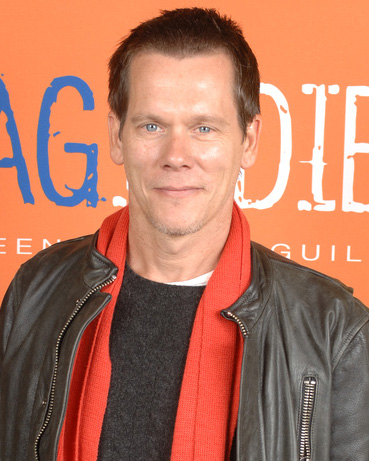
\includegraphics[scale = .4]{Kevin_Bacon.jpg}
\caption{Kevin Bacon TODO: From wikipedia source it correctly}
\end{figure}

Kevin Bacon is a famous actor who has been in a lot of movies. The six degrees of Kevin Bacon came from a comment made in an interview where Bacon said that he had worked with everyone in Hollywood or someone who's worked with them.  The idea is that you can connect actors to Kevin Bacon. Each actor has a Bacon number that is found as follows:
\begin{itemize}
\item Kevin Bacon has a Bacon number  of 0
\item Actors that have been in a movie with Kevin Bacon have a Bacon number of 1
\item For all other actors $X$, if the lowest number of any actor that $X$ has been in a film with is $n$, $X$ has a Bacon number of $n+1$
\end{itemize}

\begin{figure}[H]

\includegraphics[scale = .6]{Example}
\caption{Jeffery Humphery was in End Game with Cuba Gooding Jr. who was in A Few Good Men with Kevin Bacon, so Jeffrey Humphrey has a Bacon Number of 2 TODO: Screenshot from http://oracleofbacon.org/ not sure if I have the rights}
\end{figure}

You can define a graph in the same way where each actor is a node and there is an edge between any two nodes if the actors were in a movie together. From this you can find the shortest path between any actor and Kevin Bacon. Of course this can be done with any actor and just not Kevin Bacon. There are equivalents in other fields, the most famous being the Erdos numbers, how far away you are to publishing a paper with the prolific mathematician with Paul Erdos.

\section*{Shortest Paths}

The are many ways to find the shortest Path in a graph. A Breath First Search will find it, but the BFS runs rather slow. Two Algorithms that are used the most are Djikstra's and Astar. For this lab, we are going to use the built in package NetworkX. NetworkX has lots of useful functions dealing with graphs. The downside is that it takes up lots of RAM, but its methods are blazing fast. To make an undirected graph you do the following:

\begin{lstlisting}
import networkx as nx
G=nx.Graph()
\end{lstlisting}

You to add nodes you use the \li{add_node(x)} method where x is the node you want to add and to add an edge you use the \li{add_edge(x,y)} method where x and y are previously added nodes. There are also \li{has_node(x)} and \li{has_edge(x,y)} that tell you if the node or edge is already added.

\begin{lstlisting}
G.add_node(x)
G.add_edge(x,y)
\end{lstlisting}

The data we are giving you list the movie and then the actors separated by '/'. Each line is a different movie.  The method \li{f = open(filename, 'r')} will open the file. \li{f.readline().strip().split('/')} will read ina line of the file and make a list seperating the actors and the movie (the movie will be the first entry). When you are done with the fileclose it with\li{ f.close()}

\begin{problem}
Write a function that loads the text file into the graph. Also build a dictionary where the key is the actor and the values are the movies that the actor was in.
\end{problem}

The method \li{nx.shortest_path(G,x,y)} outputs a list that is one of the shortest paths between x and y and \li{nx.shortest_path_length(G,x,y)} outputs the length of the shortest path.

\begin{problem}
Find the shortest path between Bacon, Kevin and Davis, Rosemary (II). Also output the movies that connect to each actor in the path. 
\end{problem}

The method \li{nx.shortest_path(G,x)} finds all the shortest paths between x and every node in the dictionary. The output is a dictionary where the nodes are the keys and the values are the shortest path between x and the node. For \li{nx.shortest_path_length(G,x)} the keys are the same but the values are the lengths between x and the node.

\begin{problem}
Find the average Bacon number for the graph. 
\end{problem}

